\documentclass[10pt, letter,twocolumn]{IEEEtran}

\usepackage{graphicx}
\newcommand{\bigO}{\ensuremath{\mathcal{O}}}
\usepackage[center]{caption}
\newcommand{\doctitle}{%
Computational Creativity/Modeling and Design}
\usepackage{textcomp}
\usepackage{listings}
\usepackage{comment}
\usepackage{fancyvrb}
\usepackage{booktabs}
\usepackage[usenames,dvipsnames]{color}
\usepackage{hyperref}
\usepackage{algorithm}
\usepackage{algpseudocode}
\hypersetup{
  colorlinks,
  citecolor=Violet,
  linkcolor=Black,
  urlcolor=Blue}
  
\begin{document}

\title{Poetry Framework: Recognize Generate and \textsc{Understand} Poetry}
	\author{\IEEEauthorblockN{Arvind Krishnaa Jagannathan, Greg Cobb,
	Michelle Scott, Sonal Danak} 
	\IEEEauthorblockA {
	\\[0.5cm] \textbf{\doctitle} \\
	\textsc{\textbf{Deliverable \#2:}}
	}
	}
\maketitle
\thispagestyle{empty}
\section{Problem}
Our problem statement was pretty well-formed right before the first deliverable. Our lofty goal is to be able to architect a framework which has the basic structures of poetry encoded in it. By that we mean that our system will be able to discern poetry from ordinary prose, recognize the structural differences which determine the type of a poem and use this knowledge to categorize different poems which are given as input. By having an ``understanding'' of the processes involved in creating poetry, our framework will also have a module/sub-system which can generate poetry. As we had mentioned in deliverable 1, the generation sub-system could utilize different corpora of text data, such as Wikipedia articles, a user's Twitter feed and so on to obtain rhyming pairs of phrases to produce a rudimentary poem.

Although the core of our project's problem statement has not evolved, in the duration since the last deliverable, we have been able to redefine the scope of each of these sub-components of the framework, including the component which is responsible for assisting a novice poet in coming up with a ``first draft'' poem.

\subsection*{Core Framework}

The heart of our system is the core poetry framework which contains rules, definitions and syntactic structures which are unique to poetry of a particular form. This framework will consist of a rule engine, which for the moment will constitute a simple rule base containing information such as rhyme scheme, meter, syllable count for a number of different categories of poetry. Right now we plan to manually populate this rule base, by considering the structures of simple poetry such as haiku, couplet and limerick. These three types of poems are fairly straightforward and we can represent them by extremely simple production rules. We hope to keep this rule base as open-ended and extensible as possible so that we can incorporate more complex rules for higher order poems such as sonnets, ballads, odes and so on. 

We realize that it will not be possible, in the first pass, to have a knowledge base covering several types of poem categories. This is the reason we have chosen the most simplest types of poems to work with during the first iteration of development. We discovered during the project meetings, that it is best to have a simple model of our vision of the framework up and running; we can always expand its breadth in future iterations.

\subsubsection*{Poetry Rule Engine}
The poetry \textit{rule engine}, is what we call the central knowledge base of our poetry framework. Currently, we plan to construct this knowledge base as a set of first-order logic (FOL) based rules for different types of poems. We chose to adopt this method during the development of the initial prototype, because the poetry we will initially deal with (haiku, couple and limerick), are characterized by their unique and rigid structural features. For instance, a simple characterization of a haiku is,\\
 $\forall x(Haiku(x)) \Longrightarrow Len(Line_1(Haiku(x)))=5 \wedge Len(Line_2(Haiku(x)))=7 \wedge Len(Line_3(Haiku(x)))=5$\\
where $Len()$ is a function which corresponds to the number of syllables in a particular line of given poem. Our decision to implement the structure of a poem in first-order logic has some obvious benefits,
\begin{itemize}
	\item It has the right balance of simplicity/clarity  vs. expressiveness. For example, a simple regular expression would suffice, if there was no counting involved. Even if counting was involved, a slightly complicated regular expression would suffice; except for the fact that the counting involves syllables and not simple words.
	\item It is very close to the implementation language. For simple poetry types like Haiku, the FOL representation is almost like a pseudo-code for the program.
	\item It is easily extensible, which is a major design objective for our team. More sophisticated rules/patterns can be incorporated by more and more complex propositions within the FOL framework.
\end{itemize}
Another example of FOL for a couplet would be, \\
$\forall x,y Couplet(x,y) \Longrightarrow Rhyme(LastWord(x), LastWord(y))$
Obviously the rules for a limerick are slightly more complex that for a couplet and a haiku, but it is still possible to represent them in a flexible and clear-to-understand manner.
\subsection*{Poetry Recognizer}
We envision the poetry recognizer component of our system to perform the following main tasks:
\begin{enumerate}
	\item Given a poetry as input (either scrapped from the web, or written by a pseudo-amateur poet), the poetry recognizer must be able to ``realize'' that the input is in fact poetry and also give the category of poems it belongs to. For now, we restrict our input to the three simple cases mentioned earlier.
	\item Given a corpus of textual data (we intend this data to be of the order of a few mega bytes atleast), the crawler part of the recognizer component would search this corpus and try to identify simple ``hidden'' poems in it (A ``hidden'' poem is a sequence of continuous sentences which fit the rhyme scheme or structure of a particular type of poem). Just based on the laws of probability, strings of words in such a large piece of prose should match the structure of a poem. This can be seen as applying the propositions in ``reverse'', i.e., codify the sentences in the corpus in a standard format and then apply backward chaining over these propositions to identify if the pre-conditions for a particular poem category (for instance a Haiku, whose conditions were mentioned above) is present. This is probably a very computationally intensive process, and was one of the ``limiting'' factors which influenced our decision of simplifying the list of poem categories under consideration.
\end{enumerate}
\subsection*{Poetry Generator}
The second component of our system is the poetry generator. We want to make this component as autonomous as possible. There are three stages of autonomy we would like to achieve here (hopefully we will be able to reach atleast the lowest level). In order of increasing autonomy these stages are,
\begin{enumerate}
	\item Given a large corpus of text, try to find words when strung together in some arbitrary sequence produce poetry. This is different from the second task of the poetry recognizer since the ``search'' across the available text is more unconstrained (as lines of the poem need not appear from adjacent sentences of the text). In this task however, we would like to try out a number of different corpora (or maybe one giant mixed corpus consisting of sum random combination of all the corpora we considered) as ``inspirations'' for the generator component. This is least autonomous, since it is very clear that this process does not appear to be particularly ``creative''.
	\item Generate a poem based on a given topic. For instance, the generator can be given a Wikipedia article's title as the topic, and then has to ``create'' poetry using this title as the theme and the words contained in that article as a candidate corpus. As of now, we have restricted our scope to just Wikipedia, but it would not be hard to imagine to extend the corpus to include other freely available online sources as well. We believe this is slightly more creative, because the generator is just constrained by the theme of the poem, and has potentially infinite combinations of words, rhyme patterns, meter etc., to choose from to create a poem.
	\item At the highest level of autonomy, we expect the poetry generator to come up with arbitrary poems, which could be a haiku, a limerick or a couplet. Were it not known to the outside world that it is a computer program, this stage should a verse quality comparable to an amateur poet.
\end{enumerate}
Note that although the third task seems the ``most'' creative, it is possibly the easiest to achieve, because it is fairly straightforward to create a couplet by taking two completely unrelated sentences, whose last words rhyme with one another. This made us realize that our generation framework needs to incorporate meaning into the verse, in two senses:
\begin{enumerate}
	\item The final poem generated needs to be ``meaningful''. This can be accomplished by means of a simple Turing test - simply hand in the poem generated by this component, and poem written by an amateur poet to a neutral observer; if the observer is able to discern the two clearly then our generator component has failed the test. A more quantitative approach would be to measure the perplexity of the word sequences generated in the final poem. Perplexity (a measure of how probable a set of words $x_1, x_2, ....x_n$ are) is given by the formula, \\ 
	$P = 2^{-\sum_x p(x) \log p(x) }$
	\item However, in order to generate meaningful poetry, the corpus cannot be simply raw text. We plan to utilize \textit{n-gram} information from the textual corpus, to prune out words which hardly occur in a sequence. For example, considering bi-gram features, we will be able to conclude that although ``red'' is a frequently occurring word and ``pony'' is a frequently occurring word, the sequence ``red pony'' usually does not appear in any corpus, and so will be deemed ``meaningless''. This may seem as a potential hindrance to the creative flair of the poem generated, but since we strive only to achieve the level of quality of a novice poet, this approach seems reasonable (atleast for a first iteration). So obviously our poem generator will not produce poems like, \\
\begin{center}
	\textit{`Twas brillig, and the slithy toves\\
  	Did gyre and gimble in the wabe:\\
	All mimsy were the borogoves,\\
  	And the mome raths outgrabe.\\}
\end{center}	
\end{enumerate}

\subsection*{Poetry Assistant}
The poetry assistant component of our framework is an example of a ``human-in-a-loop'' experiment. We want this component to be a collaborative tool, which helps in enhancing the creativity of the human who is using the tool. We identified several possibilities of this tool, and have narrowed it down to the following specific use-cases:
\begin{itemize}
	\item If the human wants to generate a particular type of poetry, he/she does not have to worry about its syntax. The poetry assistant will generate a ``template'' which will highlight the property of each verse (for example the number of syllables in a line, the rhyme scheme of a a set of lines and so on). If the human violates one or more of the rules (for example if the poet types in a line with 10 syllables as the first line of a haiku), the assistant would highlight these mistakes.
	\item As an additional step, we want this AI assistant to be able to suggest alternative words in cases where the human is unable to form a correct structure of the poem using his ``current'' vocabulary of words. This step may or may not be feasible within the time-span of the project, but it is definitely a worthwhile area to investigate further.
	\item A ``highly'' optimistic ambition is to have the AI assistant actually partner the human in creating poetry. For example, if the poem were just a set of couplets, the human could type in the first sentence of the couplet, and the AI should be able to generate a \textbf{meaningful} second sentence which \textbf{rhymes} with the first. Clearly some of the challenges of the poetry generation component also need to be overcome here.
\end{itemize}

\subsection*{Creative Contributions}

The one obvious focal point of our project is to be able to write a computer program which is able to ``understand'' the nuances of the structure and semantics of poetry. By studying the different techniques involved in generating various kinds of poetry, we might be able to simulate creativity and creative behavior into an AI agent. Hopefully at the end of this project, not only would be have a pretty creative toolkit, but we would have also had an opportunity to study the cognitive processes required to construct good poetry (and therefore be able to possibly construct meta-cognitive models about human creativity). It is obvious that a very creative task such as writing poetry cannot be trivialized into a bunch of propositional rules, but our endeavor would provide a quantitative as well as a qualitative difference measure, between how a human would craft and understand poetry and how a computer (possibly) would.

\section{Architecture}
The main focus of our system architecture is centered around a central poetry recognition framework. Figure \ref{big_picture} presents a pictorial representation of the different components of the architecture and how they are related to one another.  In the following sections we present a detailed architectural description of each of the individual components of the system.

\begin{figure*}[ht]
  \centering
    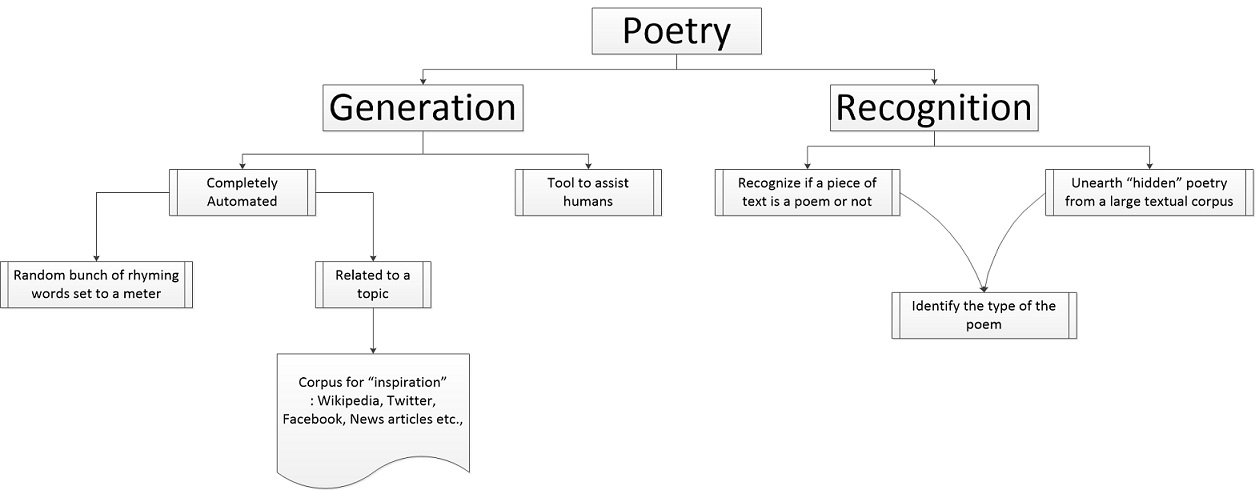
\includegraphics[scale=0.5]{Images/Big_Picture}
    \caption{Overall Scope of the Project}
  \label{big_picture}
\end{figure*}

\subsection{Poetry Recognizer}
As mentioned earlier the poetry recognizer is driven by an input of textual data. At this iteration of development, we will concern ourselves with three main stages of text processing,
\begin{enumerate}
	\item Splitting each text document into sentences. This we hope to achieve by making a very simplistic assumption that the newline character delimits a sentence.
	\item We then split the sentence into the words which constitute them.
	\item Now that we have broken down a large text document into sentences and words, it becomes more convenient for us to apply the logic rules. For instance, in order to check if this document is a haiku poem, we do the following additional (haiku-specific) steps:
		\begin{itemize}
			\item If the text document is identified to have more than 3 sentences, then it is recognized as not a Haiku poem.
			\item We utilize Python's Natural language Toolkit's (NLTK) English Word Syllable counter, to obtain the number of syllables in each word of a sentence.
			\item We add the number of syllables of each word on the first, second and third lines respectively. If these are correspondingly equal to 5, 7 and 5, the component identifies the document as a Haiku.
		\end{itemize}
	\item The above step can easily be modified to check for the existence of other types of poetry. For instance, to check if the current document is a couplet, the couplet-specific steps are:
		\begin{itemize}
			\item Obtain the last word in each of the sentences, taken two at a time. We are able to determine if two words rhyme with each other, by simply performing a look-up in the Carnegie Mellon Pronouncing Dictionary (CMUDict). If every pair of words extracted from above rhyme with one other, then the text document satisfies the condition of being a couplet.
		\end{itemize}
\end{enumerate}

A detailed architecture diagram of the recognizer component is depicted in Figure \ref{architecture}. Note that more complex rules to recognize other forms of poetry can be added to the rule base, and the procedure for ``category match'' can be tacked on to the existing architecture. 
\begin{figure}[ht]
  \centering
    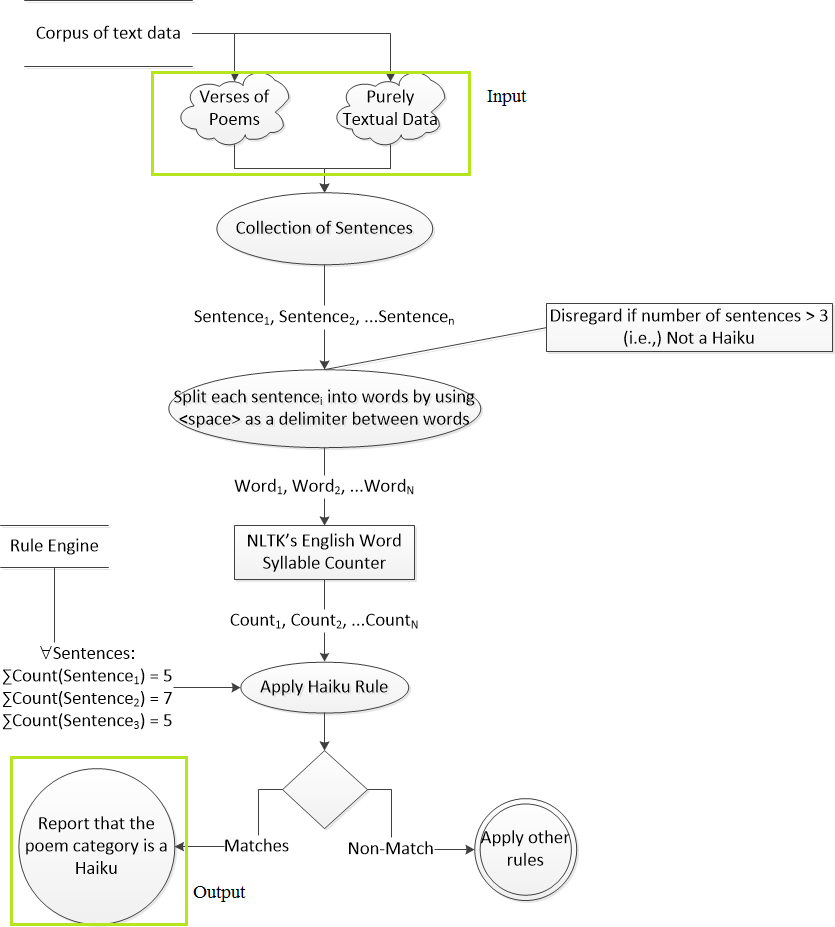
\includegraphics[width=10.3cm, height=11cm]{Images/arch1}
    \caption{Architecture Diagram for the Poetry Recognizer Framework}
  \label{architecture}
\end{figure}

A big portion of our project requires us to utilize existing domain knowledge in the field of language. The primary source of this for our project is the Carnegie Mellon Pronouncing Dictionary (CMUdict).  This dictionary provides us with all the information we need to know about words to construct many different types of poetry.  CMUdict breaks 125,000 English words into 39 phonemes.  By looking at these phonemes we can determine what words rhyme with each other.  Breaking the words into phonemes also gives us the potential to explore more advanced poetry concepts like slant or internal rhymes. CMUdict also gives information about the lexical stress of the phonemes, which allows us to use the information for poetry elements like meter.  

\subsection{Poetry Generator}
The poetry generator component of our framework, performs a very statistical analysis of the text corpus presented to it. There are two sub-components of the generator module, which takes in a text corpus and uses only the words exclusively in that corpus to generate poems. The both have a similar underlying architecture, presented in Figure \ref{architecture2} and described below.
\begin{figure}[ht]
  \centering
    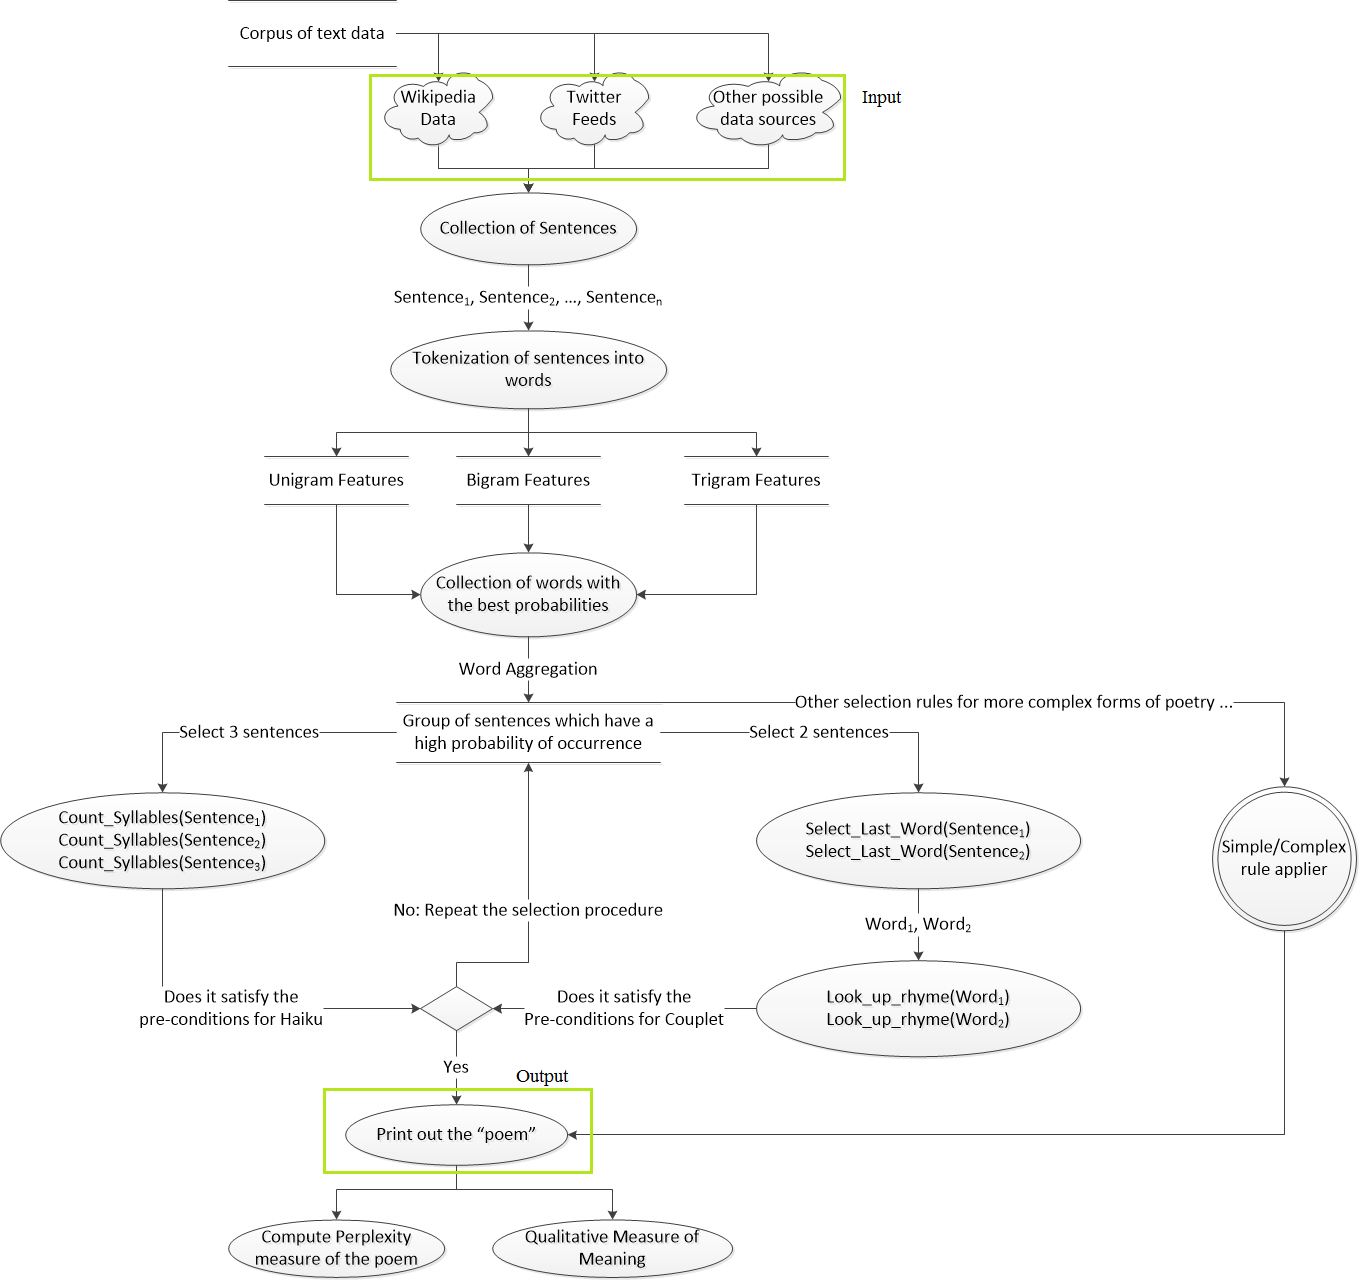
\includegraphics[width=10.3cm, height=11cm]{Images/arch2}
    \caption{Architecture Diagram for the Poetry Generator Framework}
  \label{architecture2}
\end{figure}

\begin{enumerate}
\item The text documents from the corpus will be stored in a bag-of-words model. This makes it easy to compute the necessary unigram, bigram and trigram feature probabilities which will be used later in the generation stage.
\item The documents are then parsed into a collection of sentences, followed by splitting up the sentences into words.
\item We will then be collecting the unigram, bigram and trigram probabilities of all possible words, word-pairs and word-triplets. This can be computed very simply as, \\
$P(word) \gets \frac{Count(word)}{Count(Words)}$ \\[0.3cm]
$P(word_{i+1} | word_i) \gets \frac{Count(word_{i+1}, word_i)}{Count(Bigrams)} $ \\ [0.3cm]
$P(word_{i-1} | word_{i,i+1}) \gets \frac{Count(word_{i-1}, word_{i,i+1})}{Count(Trigrams)}$ \\ [0.3cm] 
\item Then we have a module which gets this probabilistically sorted collection of words, and constructs random sentences out of them. Initially we plan to have an upper and a lower limit on the length of each sentence.
\item The above is a computationally expensive step, since there are, combinatorially, several ways of forming arbitrary length sentences from a potentially large group of words.
\item Once we generate the list of candidate ``verses'', depending on the type of poem to be generated, we select a limited subset of the candidate list.
\item The rule engine is applied on the candidate list, to verify if it matches the structure and semantics of that category of poetry.
\item If it does not, we try again, until a set of sentences corresponding to the patterns defined in the rule engine are found.
\item To measure the meaningfulness of a poetry, we calculate the \textit{Perplexity} (defined earlier) of each sentence. NLTK's \emph{ngram} package provides the functionality of computing the perplexity (as $2^{Cross\_Entropy}$) of a given text. We measure the \textit{Perplexity} score of the entire poem as a product of the \textit{Perplexity} of each ``verse'' in the poem. That is, \\
	$P(poem) \gets \prod_i P(sentence_i)$
\item The perplexity measure is a simple quantitative measure of a poem's meaning. However, a work of art, such as a poetry, need to be also judged for its quality. Since there is no better judge of quality of art than a human, we propose to have a human judge the poem generated by the system for its lyrical content.
\end{enumerate}
It is quite apparent that we might not be able to achieve the levels of creativity as say Robert Frost, but we hope to achieve parity to the level of a first-time or a novice poet.

The third sub-part of the poetry generator component, generates random poetry without any restrictions on the vocabulary to be used in the lines. Here in addition to the criteria of each line being meaningful, the entire poetry as a whole must have some common underlying theme (this is also a constraint with the first two categories of generators, but more so with the fully autonomic version). In the first iteration of our project, we will be implementing this as a slight modification of the first two sub-parts. 
\begin{itemize}
	\item Since we already have Wikipedia articles as a data source, the theme of the poem-to-be, would be selected as one of the titles.
	\item However, instead of constraining ourselves to the words in the Wikipedia article, we will utilize a lexical database such as WordNet, to generate synonyms of some of the most important terms within the document. 
		\begin{enumerate}
			\item To identify important words in an article, we will be constructing an inverted index of every word (= 1/count(word)) in that document. Words who have an inverted index within an empirically established threshold will be deemed important.
			\item However, to get a quick and dirty version of our generator running, we might add in extra manual annotations to certain words in the article, for which synonyms will be looked up in WordNet.
			\item The words in the Wikipedia article along with the synonyms from WordNet would be added to the corpus of words for the ``base'' generator framework.
		\end{enumerate}
		\item We apply the same sequence of steps as previously described on this modified corpus.
		\item We might insert certain pseudo-random equivalent perturbations in the words of the generated poem. For instance, if the poem is a haiku, we might substitute at random, a word with $k$ syllables with a ``related'' word also of $k$ syllables.
\end{itemize}
Clearly, to generate a poem completely autonomously, enormous amounts of lexical and domain knowledge is necessary about words, their meanings and their associations with one another. We will be primarily be looking towards WordNet as the source of this semantic information. The system architecture is shown in Figure \ref{architecture3}

\begin{figure}[ht]
  \centering
    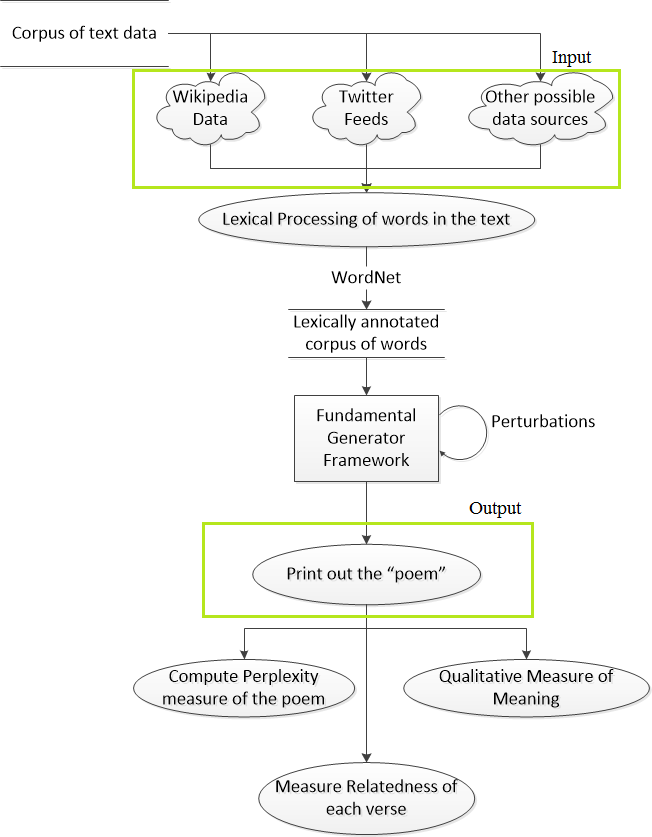
\includegraphics[width=7cm, height=8cm]{Images/arch3}
    \caption{Architecture Diagram for the Completely Autonomous Poetry Generator Framework}
  \label{architecture3}
\end{figure}

We also plan to integrate other categories of poetry, along with the ability to define one's own custom rhyme scheme, meter and syllable count, once we get the basic framework to work.

We also have some enhancements planned, which time-permitting, we would like to try out. One immediate addition would be to use certain words in the article as ``key terms'' and use a web crawler to find words which occur frequently with these words. Another is to utilize a semantic thesaurus, which does not provide a raw list of synonyms to a word given as input, but instead filters them by their sense and context. Expert poets construct creative metaphors for words, use words in contexts unimaginable to people with lower degrees of command over the language. A major effort is required to codify such actions which appear to be  ``magical'', retrieval of wildly obscure words which seems ``automatic'' into algorithms and data structures. However, after multiple discussions we have decided to approach this problem with a smaller scope, and build on it as and when a good portion of the pieces are in place.

\subsection{Poetry Assistant} 
The poetry assistant component is the most nascent part of our framework. There are two sub-parts to the assistant. One is a templating tool, to generate a skeletal structure for a particular poem. This will help first-time poets to direct their focus on semantics rather than syntax. For the three categories of poems that we have decided to work with, it is pretty straight-forward to construct an outline (due to the fact that a haiku, couplet and limerick follow very simple structures and rhyme scheme). However, the most difficult part of writing a poem is to conjure words which fit into the context of the poem. We hope to address this with the second part of our assistant: an automatic word suggester. The words suggested would need to satisfy two primary constraints,
\begin{enumerate}
	\item Fit into the meter and rhyme scheme of the poem. For instance, if the human poet is struggling to complete a couplet, the assistant will be able to suggest words which rhyme with the last word of the first verse in the couplet. This is fairly straightforward by performing a look-up in the CMUDict.
	\item Fit into the overall scheme of the poem's vocabulary - the words need to be semantically related. Again we plan to utilize WordNet's semantic lexicon for this purpose.
\end{enumerate}
Clearly, both the above requirements are also implicit in the generator and recognizer components. Thus the poetry assistant's architecture can in fact be visualized as a subset of features of the two previously described components, which is what is shown in Figure \ref{architecture4}. The property of a line of poetry is given in parenthesis next to it.

\begin{figure}[ht]
  \centering
    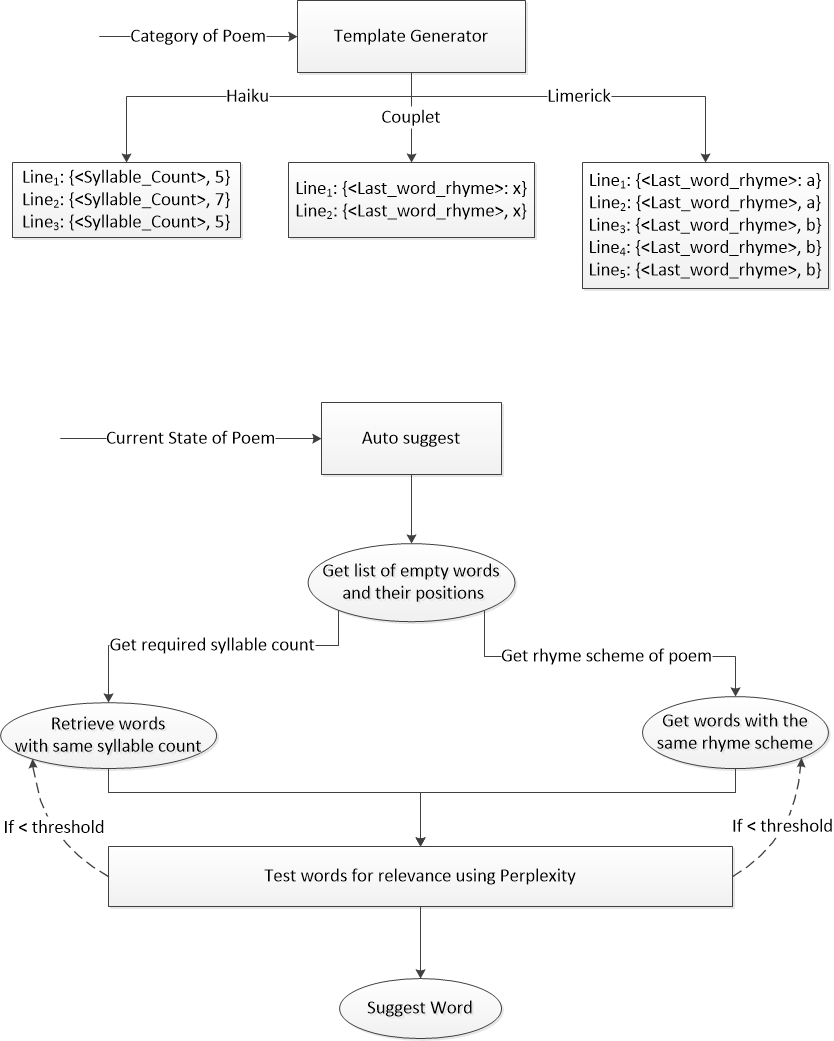
\includegraphics[width=7cm, height=8cm]{Images/arch4}
    \caption{Architecture Diagram for the Poetry Assistant}
  \label{architecture4}
\end{figure}

As it might have been obvious from the description of the architecture, several requirements of the framework are common across the three components. A bird's eye view of all the possible classes across components, and their relations and interactions among them are summarized in Figure \ref{class1}.

\begin{figure*}[ht]
  \centering
    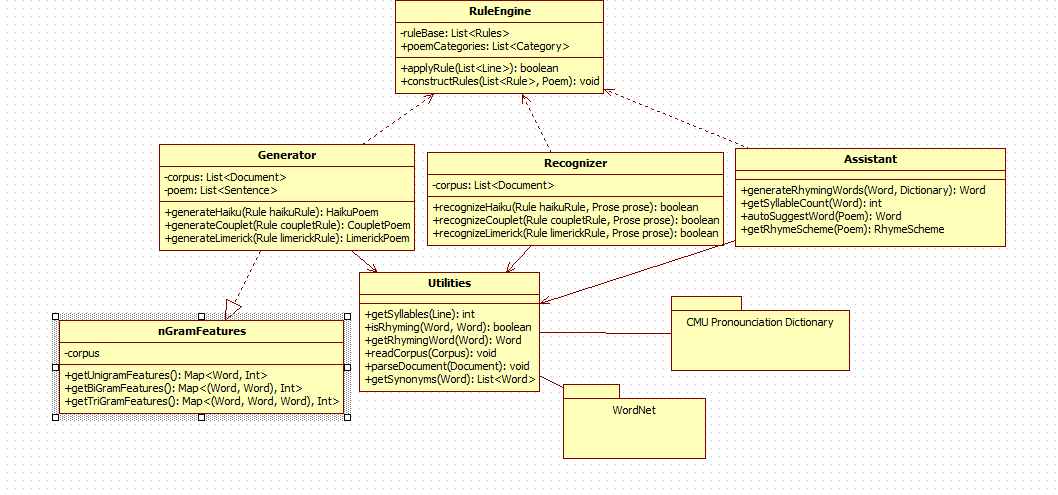
\includegraphics[scale=0.5]{Images/class1}
    \caption{Relation between different classes within the framework}
  \label{class1}
\end{figure*}

\section{Data Structures}
\section{Algorithms}
\section{Interface Diagram}
In this section we list out the mockups which we have come up with for the user interface of our application. The figures appearing in this section are as follows:
\begin{itemize}
\item Figure \ref{gui1} shows the user interface of the main application. Here a user will be able to pick which of the available components he/she wants to use.
\item Figure \ref{gui2} allows the user to take either a corpus of documents as input or paste some text and then search for poems within it.
\item Figure \ref{gui3} presents the generator component. This is a preliminary mockup, which displays a barebones interface. The human can select the rhyme scheme and the category of the poem along with its meter. The GUI depicts the third level of autonomy - generate the poem without any ``inspirational'' text corpus.
\item Figure \ref{gui4} is the poetry creation assistant. As shown in the figure, the assistant suggest words which will be a ``good'' fit into the empty spot, based on the rhyme scheme desired by the user.
\end{itemize}

\begin{figure}[ht]
  \centering
    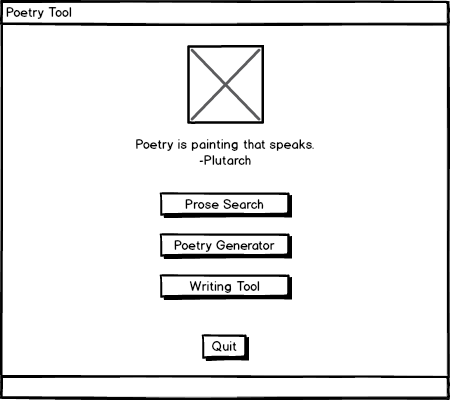
\includegraphics[scale=0.5]{Images/Main}
    \caption{Mockup of the ``main'' GUI window}
  \label{gui1}
\end{figure}

\begin{figure}[ht]
  \centering
    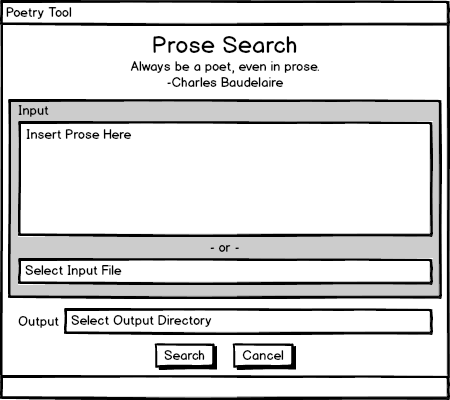
\includegraphics[scale=0.5]{Images/recognize}
    \caption{Mockup of the Recognizer component}
  \label{gui2}
\end{figure}

\begin{figure}[ht]
  \centering
    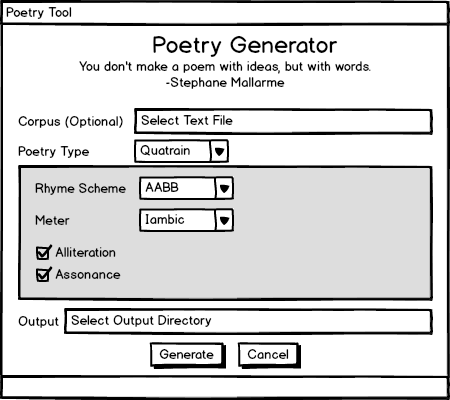
\includegraphics[scale=0.5]{Images/generate}
    \caption{Mockup of the Generator component}
  \label{gui3}
\end{figure}

\begin{figure}[ht]
  \centering
    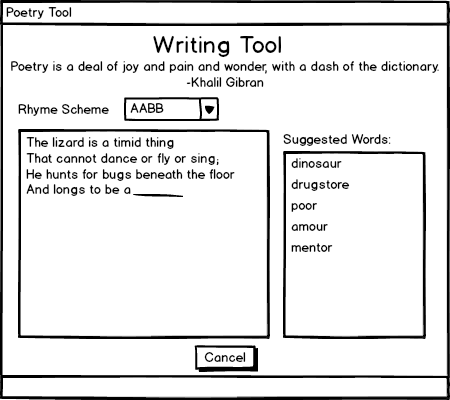
\includegraphics[scale=0.5]{Images/tool}
    \caption{Mockup of the Poetry Assistant component}
  \label{gui4}
\end{figure}

Note that our first iteration of this project will likely not have a graphical user interface, since it is an abstract software framework.  Since the discoveries we make while working on the framework will shape our final product, it is hard to predict exactly what the interface will look like.  However, based on our early ideas for potential project paths, we developed these user interface mockups to show what our product could end up looking like.


\bibliographystyle{unsrt}
\bibliography{myrefs}
\end{document}
\end{document}